Afin de mener à bien l'objectif énoncé dans l'introduction, les robots doivent se comporter de manière intelligente. Le plus important est l'interaction avec l'environnement. En effet, le choix de la bonne action est cruciale. Il est cependant délicat de définir une seule <<meilleure>> action. Ceci est développé plus bas, en introduisant le concept de \emph{rationalité}. 
De manière générale, un robot peut être assimilé à un agent qui reçoit des \emph{percepts} par l'intermédiaire de ses capteurs. L' \emph{agent} réagit alors en exerçant une action sur l'environnement grâce à ses \emph{effecteurs}.
\begin{figure}[h!]
  \centering
  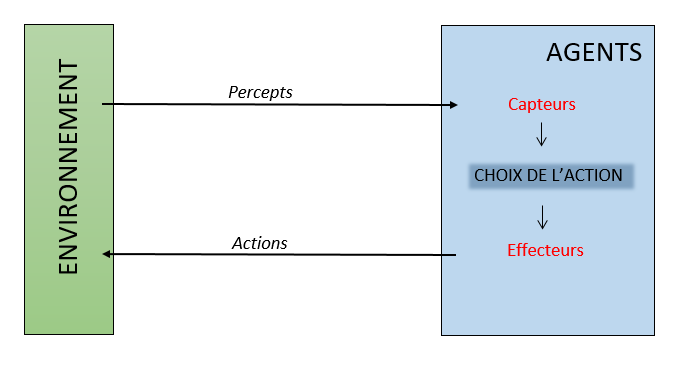
\includegraphics[width=0.7\textwidth]{cycleInteractionAI.png}
    \caption{Cycle d'interaction entre l'environnement et les agents}
\end{figure}
La description des différents capteurs et effecteurs du robot est faite dans le chapitre \ref{chap:argosFootbot}.

Comme énoncé précédemment la rationalité d'un agent peut être délicate à mesurer. D'après \cite{AIBrique}:
\begin{quote}
  <<La rationalité n'est pas synonyme de perfection, la rationalité maximise la performance espérée tandis que la perfection maximise la performance réelle.>>
\end{quote}


En effet, dans un groupe composé de plusieurs agents, un choix d'action peut s'avérer bénéfique pour un agent mais mauvais pour l'ensemble du groupe. C'est pourquoi il est préférable de concevoir les mesures de performance en fonction de ce que l'on souhaite obtenir dans l'environnement et non en fonction de la façon dont devrait se comporter un agent.

A partir de cela, tout problème peut être formellement défini par cinq composantes. Tout d'abord l'état initial dans lequel commence l'agent, puis la description de ses différentes actions, c'est à dire toutes les actions possibles dans un état donné. Ensuite, vient le modèle de transition, il décrit ce que chaque action réalise. Ces trois premières composantes définissent l'espace des états du système, c'est à dire l'ensemble de tous les états accessibles par une séquence d'action à partir de l'état initial.

Dès lors l'espace d'état peut être interprété sous forme d'arbre où les nœuds représentent des états et les branches des séquences d'action. Il en découle la notion de chemin représentant une séquence d'états reliés par une séquence d'action.

La quatrième composante correspond au test but. Celle-ci détermine si un état donné est un état but. Enfin vient la cinquième et dernière composante, le coût du chemin. Elle permet d'attribuer une valeur numérique à un chemin en accord avec la mesure de performance imposée.

Maintenant qu'une présentation générale de l'intelligence artificielle a été faite, le comportement d'essaim d'agents intelligents peut être étudié. Pour ce faire, il s'est avéré très intéressant d'en comprendre le comportement à partir d'exemples se trouvant dans la nature. Les fourmis et les abeilles illustrent bien cela. Deux algorithmes mettant en avant leur comportement sont présentés ci-dessous.

\section{Algorithme des fourmis}

Cet algorithme est basé sur le comportement des fourmis dont une des particularités est la communication au travers de l'environnement par dépôts de phéromones.

L'algorithme se présente de la manière suivante. Pour commencer, une exploration de l'environnement est faite par les fourmis. Si l'une d'entre elles trouve une source, elle déposera, lors de son retour au nid, des phéromones tout au long du chemin qu'elle emprunte. Dès lors, lorsque que d'autres fourmis partiront à la recherche de nourriture, elles auront tendance à suivre le chemin  marqué de phéromones. Et à leur retour à la colonie, elles renforceront cette piste \cite{wikiFourmi}.

Cet algorithme illustre une communication indirecte d'un essaim et la manière dont ce dernier est influencé \cite{communicationFourmis}. L'autre algorithme, illustrant le comportement d'une structure organisée, est l'algorithme des abeilles.

\section{Algorithme des abeilles}

L'algorithme des abeilles est un «algorithme d'optimisation basée sur un comportement intelligent particulier des essaims d'abeilles».CITATION?

Dans cet algorithme, tout comme dans celui des fourmis, les abeilles explorent le milieu environnant le nid. Par contre, ces dernières partagent des informations de manière directe. En effet, si une source est trouvée, celle-ci débutera une danse qui aura pour but d'avertir les autres abeilles. Plus la source sera importante, plus la danse sera complexe.SOURCE

Comme observé dans ces algorithmes, la communication est indispensable à une bonne organisation d'un collectif d'individus. Dans le cadre de ce projet, le moyen dont les robots vont se partager les informations peut s'y inspirer.

D'une part, en s'inspirant de la communication des abeilles, les robots pourraient communiquer l'emplacement des sources de manière directe. Pour cela, celles-ci allumeraient leur LED pour communiquer l'emplacement d'une ressource. Ou d'autre part, pour communiquer indirectement, les robots pourraient déplacer les objets à l'aide de ses effecteurs. Par exemple, ils déplaceraient les obstacles dans son environnement de telle manière à créer un chemin qui mènerait du nid à la source.

Le prise en charge de la communication des robots ne sera traitée qu'au second quadrimestre. Mais tout ceci est concevable car les robots disposent d'effecteurs capables d'interagir sur l'environnement et de capteurs capables de cerner les différentes modifications de ce dernier.